\documentclass[12pt, oneside, a4paper]{article}


\usepackage[utf8]{inputenc}
\usepackage[a4paper,margin=2cm, includeheadfoot]{geometry}
%\usepackage[a4paper,hmargin=2cm,vmargin=2.0cm,includeheadfoot]{geometry} % same as above but with separate conditions for vertical and horizontal margins

\usepackage{amssymb} %Extra symbols (such as approximately less than)
\usepackage{amsmath} %Extra maths tools (such as aligning equations)

\usepackage{graphicx}
\usepackage{setspace}
\usepackage{lipsum}
\usepackage{abstract} %Added to change abstract title size

\usepackage{booktabs}

\usepackage{fancyhdr}
\usepackage{hyperref}

%\usepackage[colorlinks=True,linkcolor=blue]{hyperref}

\usepackage[numbers]{natbib}

%\usepackage{indentfirst} %Indent first paragraphs

\usepackage{extramarks}
\usepackage[font=normalsize,labelfont={bf}]{caption} %Bolden caption titles


\usepackage{ragged2e}

\usepackage{multicol, caption, float}

\usepackage{comment}

% \usepackage{multicol}
\usepackage{multirow}
\usepackage{array}



\newenvironment{Figure}
  {\par\medskip\noindent\minipage{\linewidth}}
  {\endminipage\par\medskip}


\usepackage{caption}
\usepackage{subcaption}


\usepackage{xcolor}
\definecolor{highlight}{RGB}{49, 4, 89}
 %Includes packages
% \usepackage[numbers]{natbib}


\pagestyle{fancy}
\fancyhf{}
%\lhead{\firstleftmark} %SOLVES LEFTMARK PROBLEM
\lhead{\leftmark}
\cfoot{\thepage}

\begin{document}

%Title page

\begin{titlepage}

\centering
% \includegraphics[width=4cm]{./figures/logo}\\[2cm]

\vspace*{5cm}


\begin{center}

% \textsc{\LARGE Quantitative Research Interview Assignment}\\[1.5cm]




\textsc{\Large Quantitative Research  Coding Project}\\[0.4cm]


\newcommand{\HRule}{\rule{\linewidth}{0.5mm}}

\HRule \\[0.4cm]
\setstretch{1.8}
{\huge \bfseries Fusion Strategy Backtest Task}\\
[-0.2cm]
\HRule

\Large Kelvin Brinham

\end{center}

% \begin{flushleft} \large

\vspace{0.5cm}
\large
\href{https://github.com/kelvinbrinham/StrategyBacktest}{\color{highlight} GitHub: StrategyBacktest}



\normalsize
\makeatletter
Date: \@date


\end{titlepage}




%\clearpage %i don't know why this was needed


%ABSTRACT--------------------------------------------------------------


\restoregeometry

\setcounter{page}{4}
\setcounter{figure}{0}

\pagestyle{fancy}


%THIS SECTION MAKES A CONTENTS PAGE------------------
\pagebreak

% \tableofcontents

% \pagebreak
%-----------------------------------------------------


\section{Introduction}

In summary, this project demonstrates how a simple trading strategy can be backtested using an object-oriented Python program. This objective could be easily performed with functional programming, or even in Excel, but I created this framework as it can be easily adjusted and extended in the future. For example, It allows transaction costs to be added.

\section{Method}

To keep the report brief, explanation of the method can be found in the code doc-strings on \href{https://github.com/kelvinbrinham/StrategyBacktest}{\color{highlight} GitHub}. In addition, this report demonstrates some \LaTeX tables produced automatically by a python tool I wrote. I briefly summarise the important points as follows:

\begin{itemize}
    \item I do not allow fractional shares. As a result, the remaining allocation is held as cash.

    \item I use an initial capital of $100,000$ to ensure that the effect of buying whole shares is not significant (given the maximum share price is $< 1700$).

    \item Upon inspecting the figures of the share prices we see asset B has a fixed price. I assume it pays dividends although I do not incorporate dividends.

    \item I use a leverage of 1. My code can handle a sum of weights which differs from 1 and the option for alternate leverage could be easily added with the expected effects on results.

    \item I model monthly rebalances and daily rebalances. I take the monthly portfolio weights to remain constant during each month for daily rebalances. Therefore, rebalances occur due to changes in asset prices and net asset value (NAV).

    \item I do not incorporate the risk-free rate into shorts. I use it for calculating the Sharpe ratio.

    \item I ignore transaction costs for the initial allocation. In other words, I assume the assets are already in the portfolio on day 1. (I do this because the total transaction costs associated with initial allocation are significant).


\end{itemize}


\section{Results}
\subsection{Default Portfolio}

\begin{table}
\centering
\caption{Portfolio performance; daily rebalancing.}
\label{table:daily_rebalance}
\begin{tabular}{rrrrrrr}
\toprule
\midrule
Transaction Cost & 0.00\% & 0.30\% & 0.00\% & 0.30\% \\
Risk Free Rate & 0.00\% & 1.50\% & 1.50\% & 0.00\% \\
\hline
Total Return & 10.35\% & 10.35\% & 10.35\% & 10.35\% \\
Return (Ann.) & 7.20\% & 7.20\% & 7.20\% & 7.20\% \\
Sharpe Ratio & 1.16 & 0.92 & 0.92 & 1.16 \\
Sharpe Ratio (Ann.) & 0.98 & 0.78 & 0.78 & 0.98 \\
Volatility (Ann.) & 7.41\% & 7.41\% & 7.41\% & 7.41\% \\
Max Drawdown & 4.48\% & 4.48\% & 4.48\% & 4.48\% \\
Max Drawdown Date & 2003-08-05 & 2003-08-05 & 2003-08-05 & 2003-08-05 \\
Longest Drawdown (Days) & 107 & 107 & 107 & 107 \\
\bottomrule
\end{tabular}
\end{table}


Table~\ref{table:daily_rebalance} outlines summary portfolio performance using daily rebalances. Monthly rebalances showed similar results because the number of daily trades in-between monthly rabalance days was very small. Further, transaction costs have a minor effect due to the small number of trades overall (due to the only significant rebalances being monthly and a small change in weight even then).

I choose an example risk-free rate of $1.5\%$ because this is similar to the US 4-week treasury bond rate in 2003-04. It has the expected effect on the Sharpe ratio.

Figures~\ref{figure:Task NAV}, \ref{figure:Task underwater} and \ref{figure:Task volatility} show the portfolio value, drawdowns and volatility.


\begin{figure}
\centering
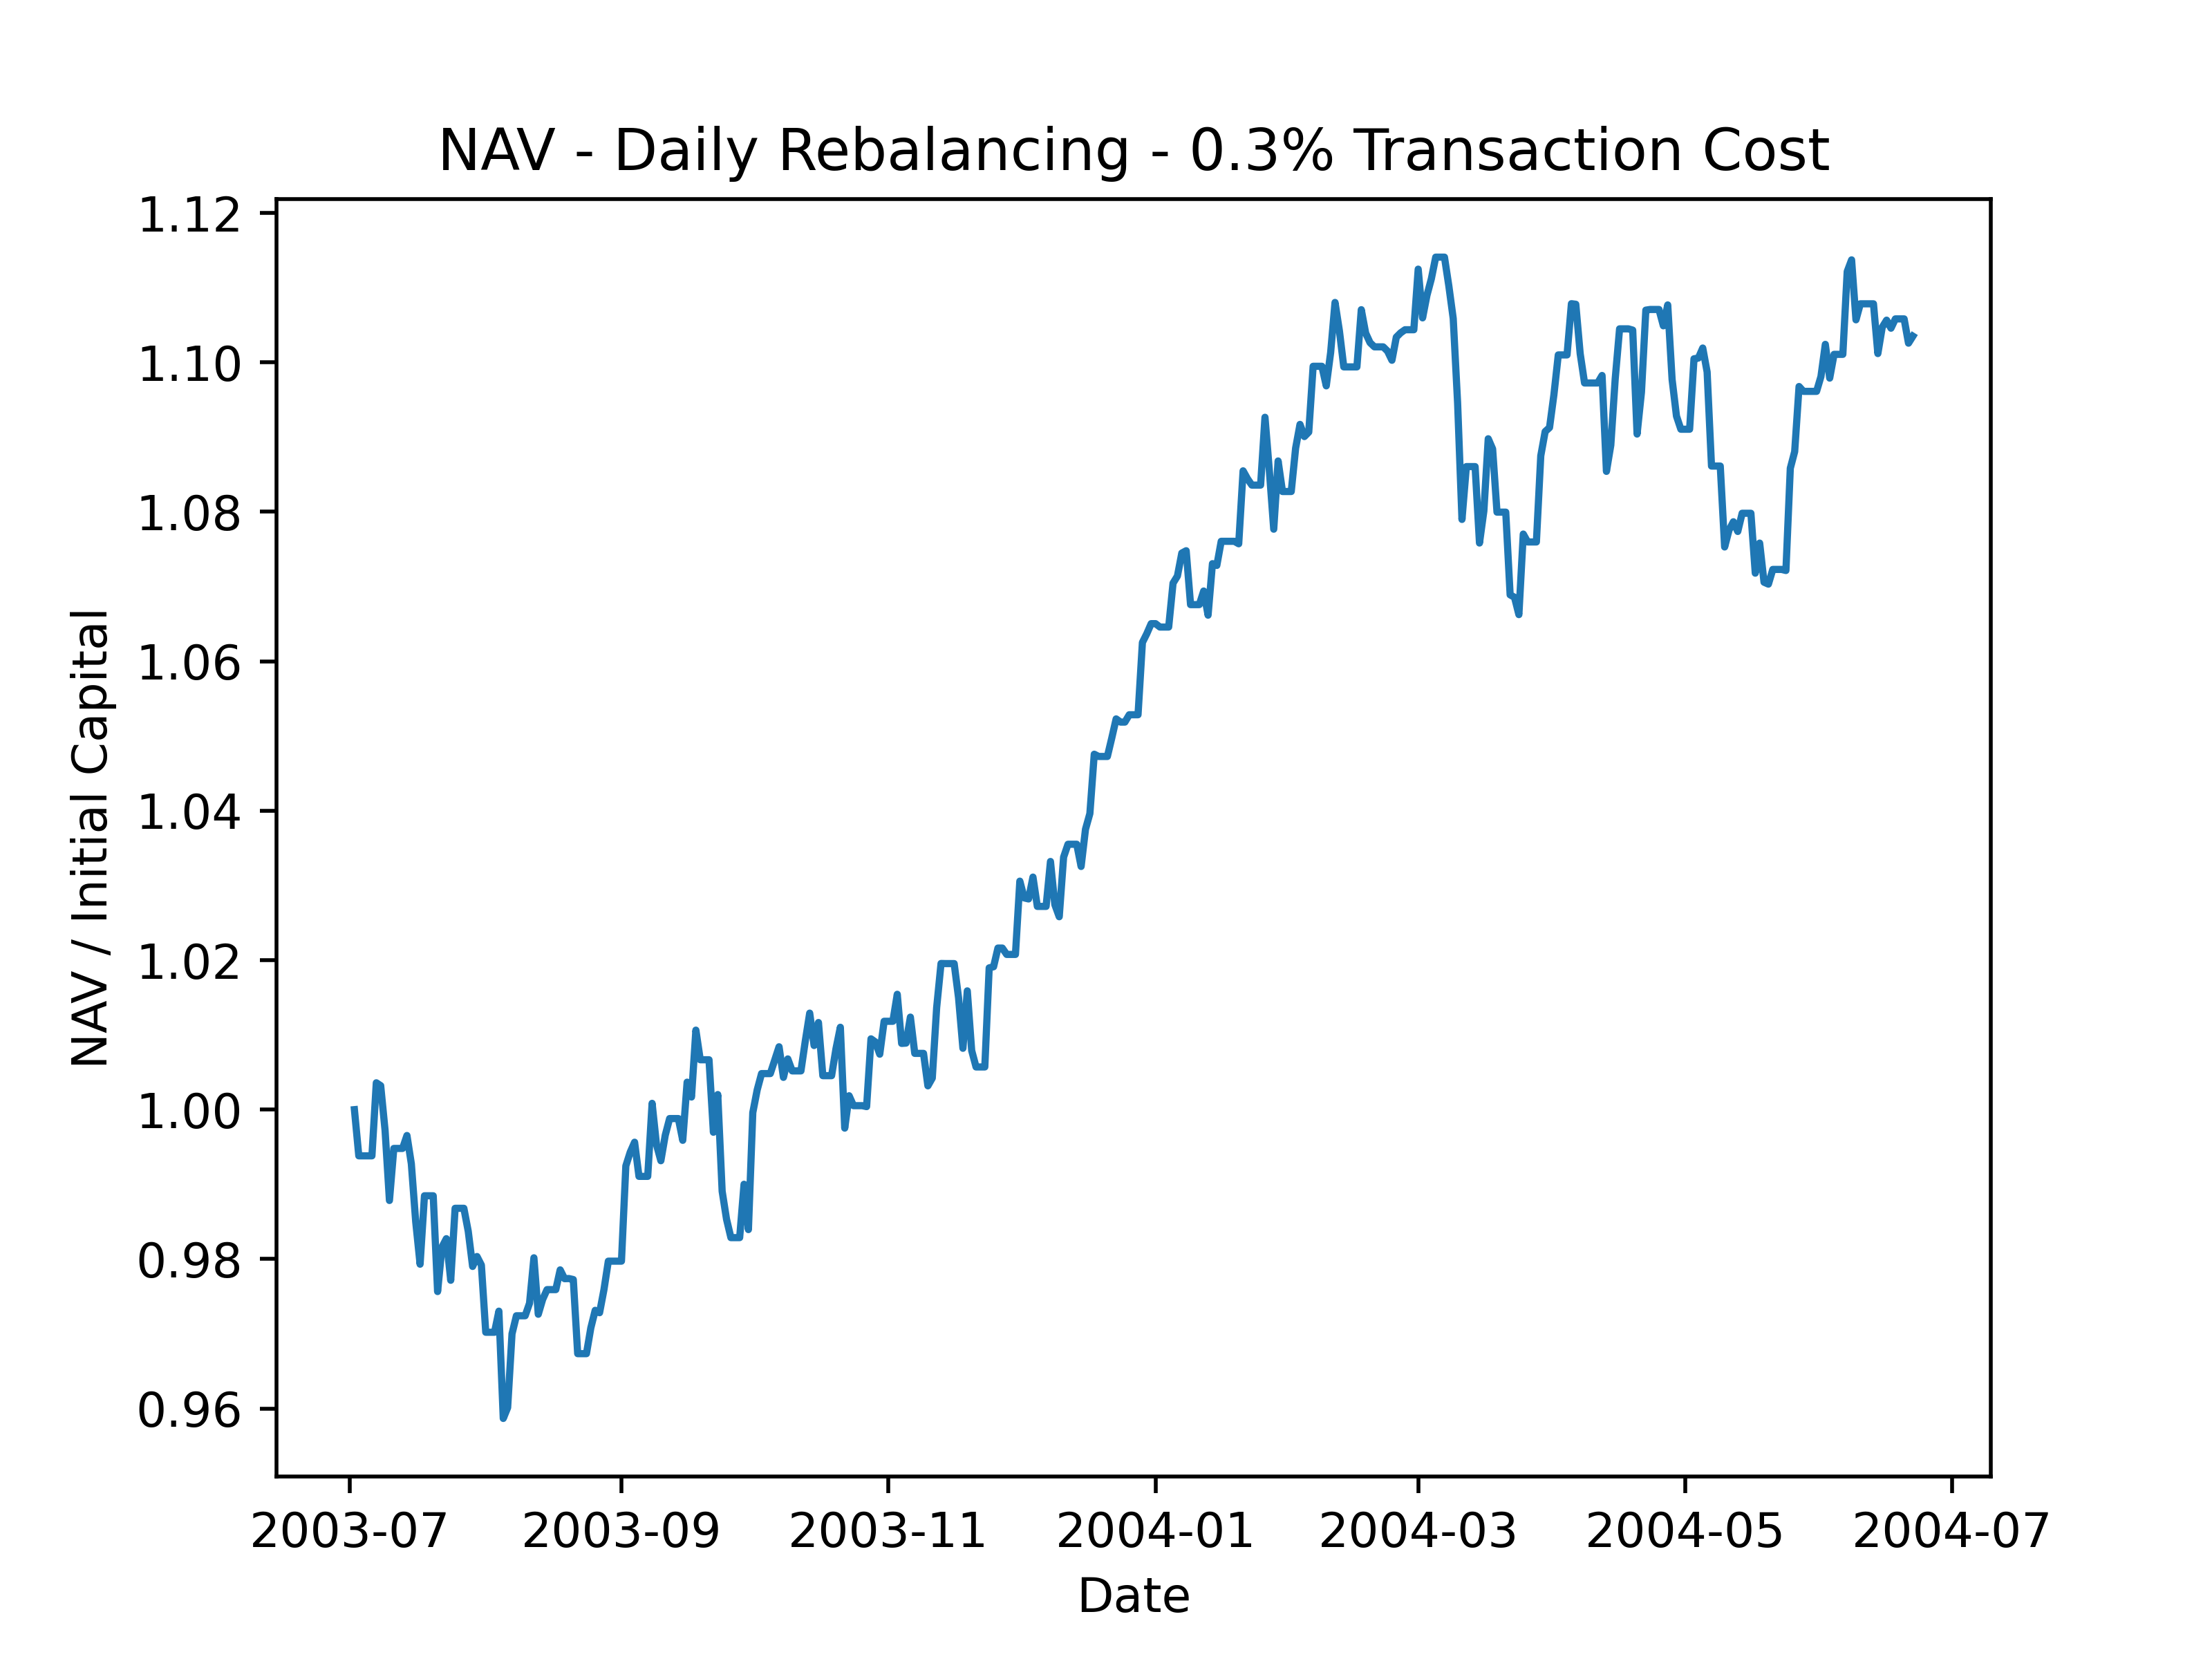
\includegraphics[width=0.7\linewidth]{./figures/nav.png}
\caption{Net asset value of default portfolio with 0.3\% transaction costs; daily rebalancing.}
\label{figure:Task NAV}
\end{figure}

\begin{figure}
\centering
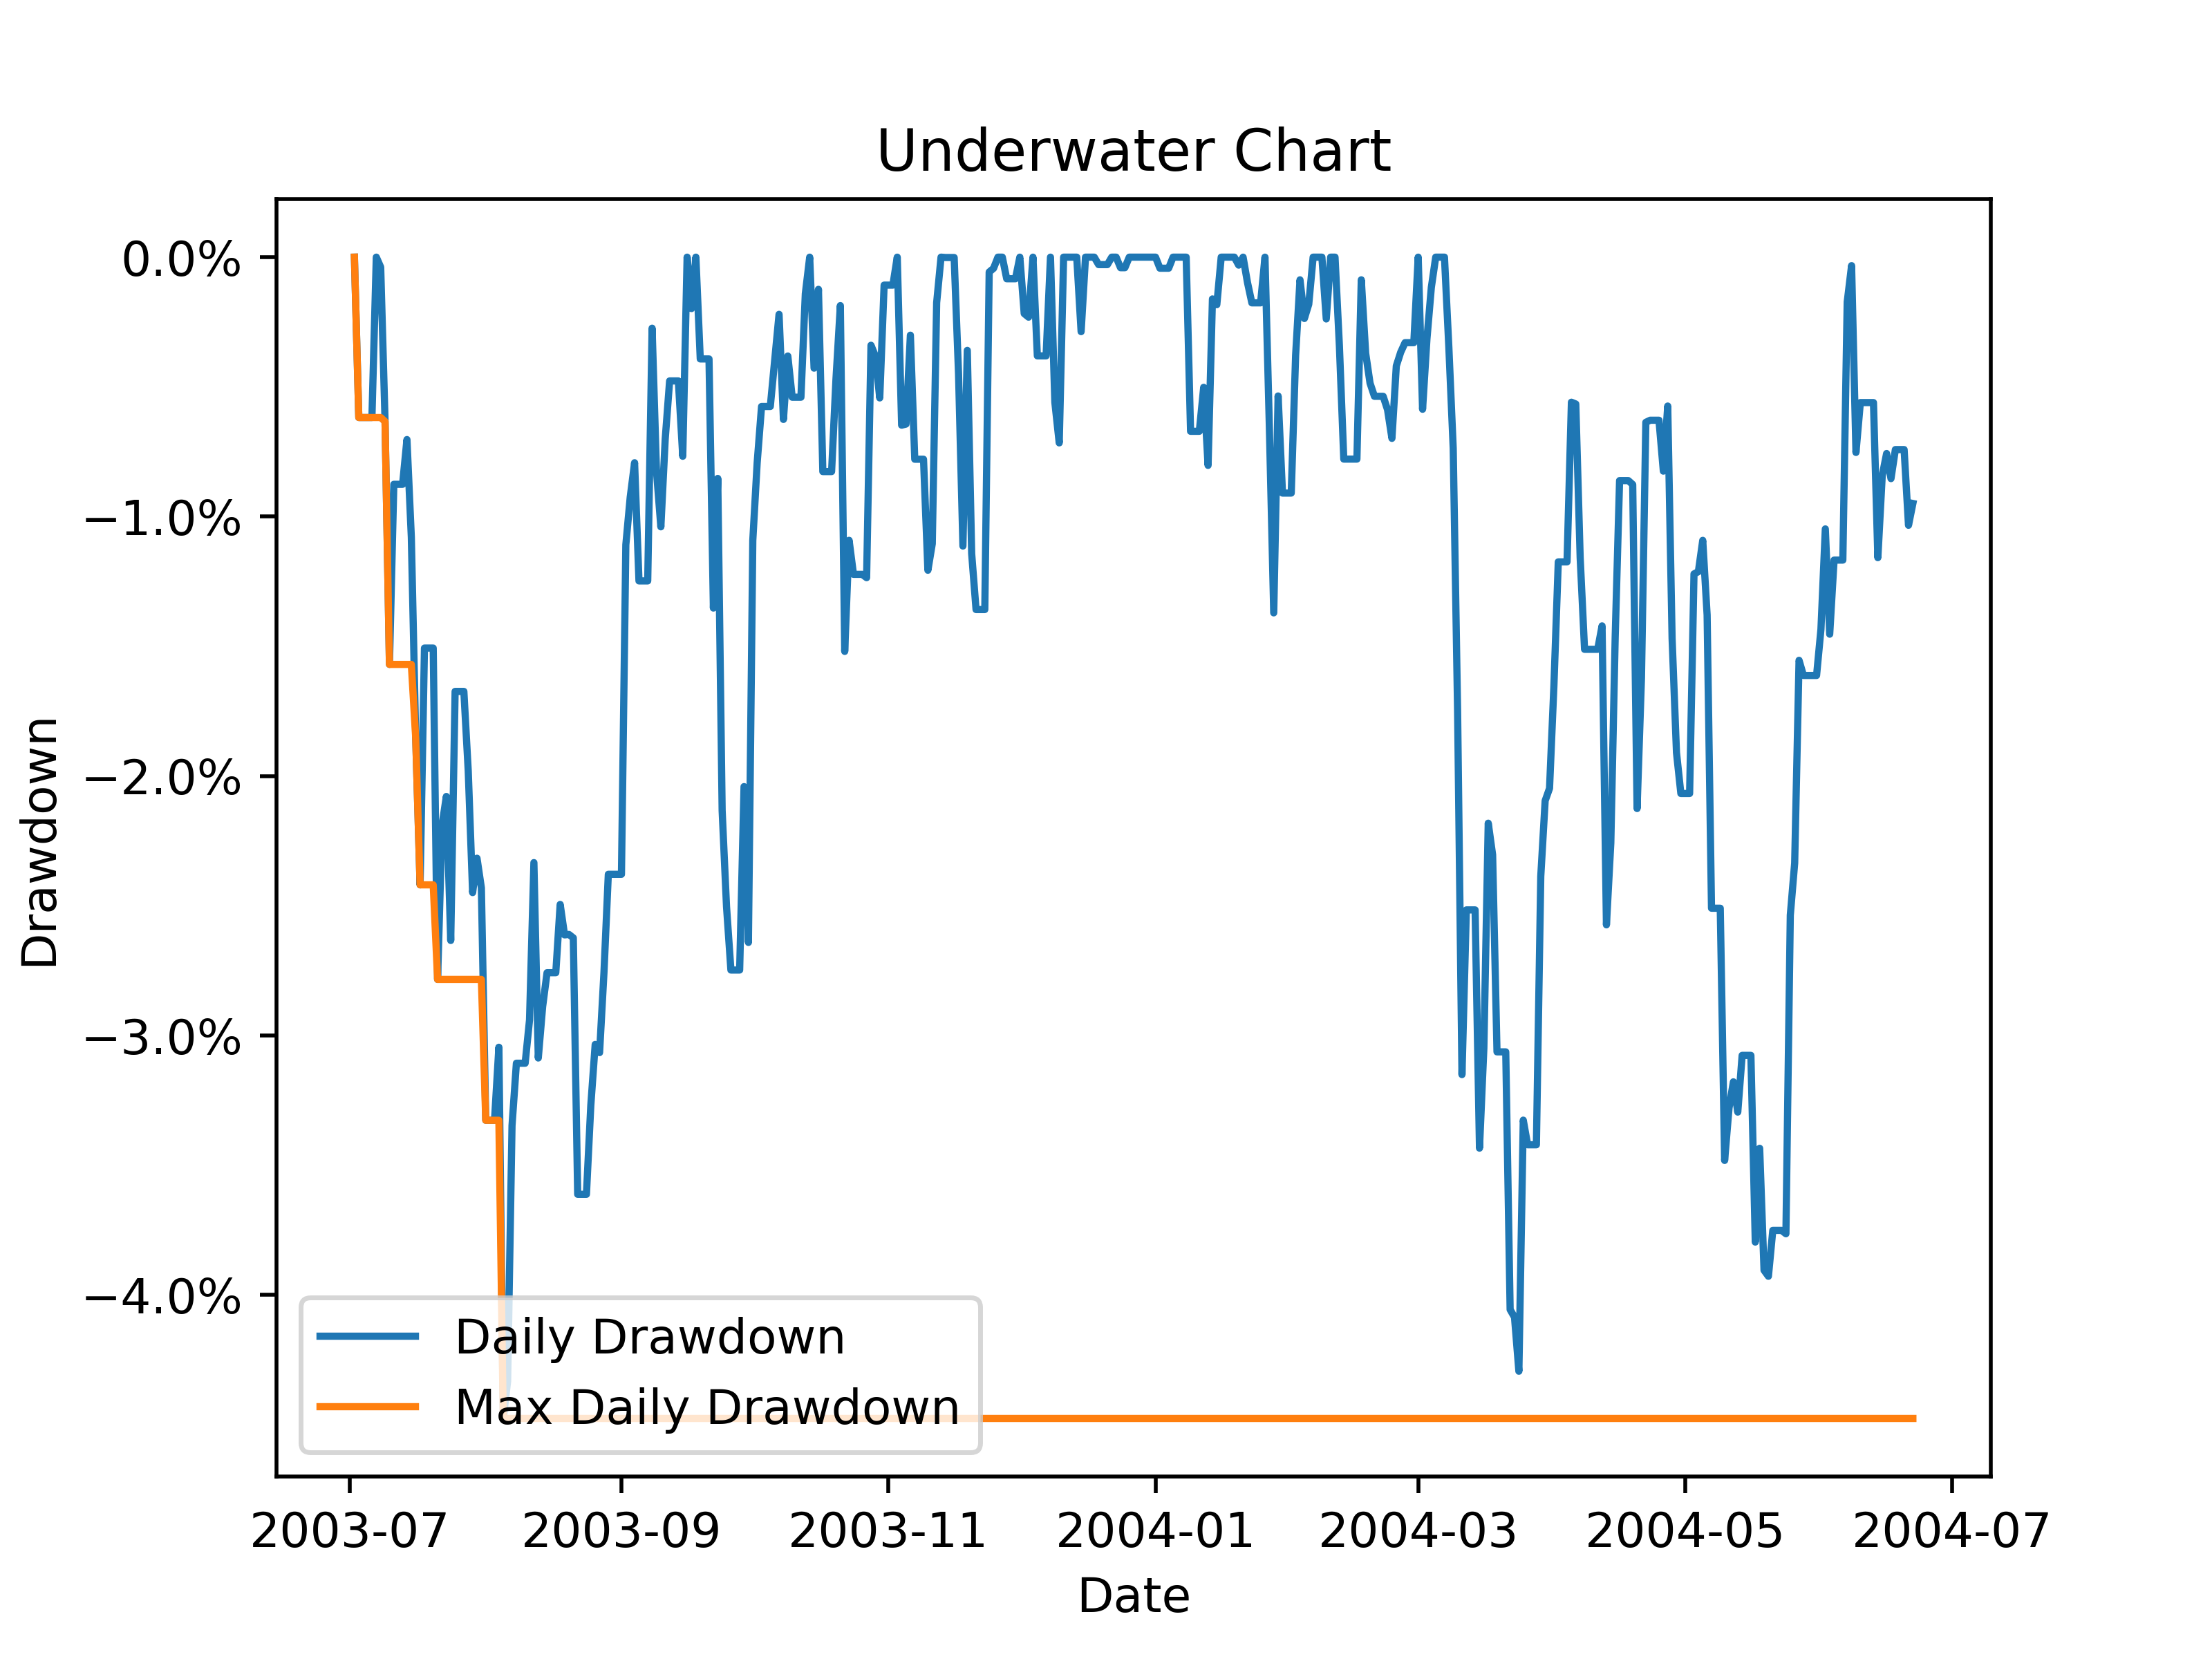
\includegraphics[width=0.7\linewidth]{./figures/underwater.png}
\caption{Drawdowns of the default portfolio with 0.3\% transaction costs; daily rebalancing.}
\label{figure:Task underwater}
\end{figure}

\begin{figure}
\centering
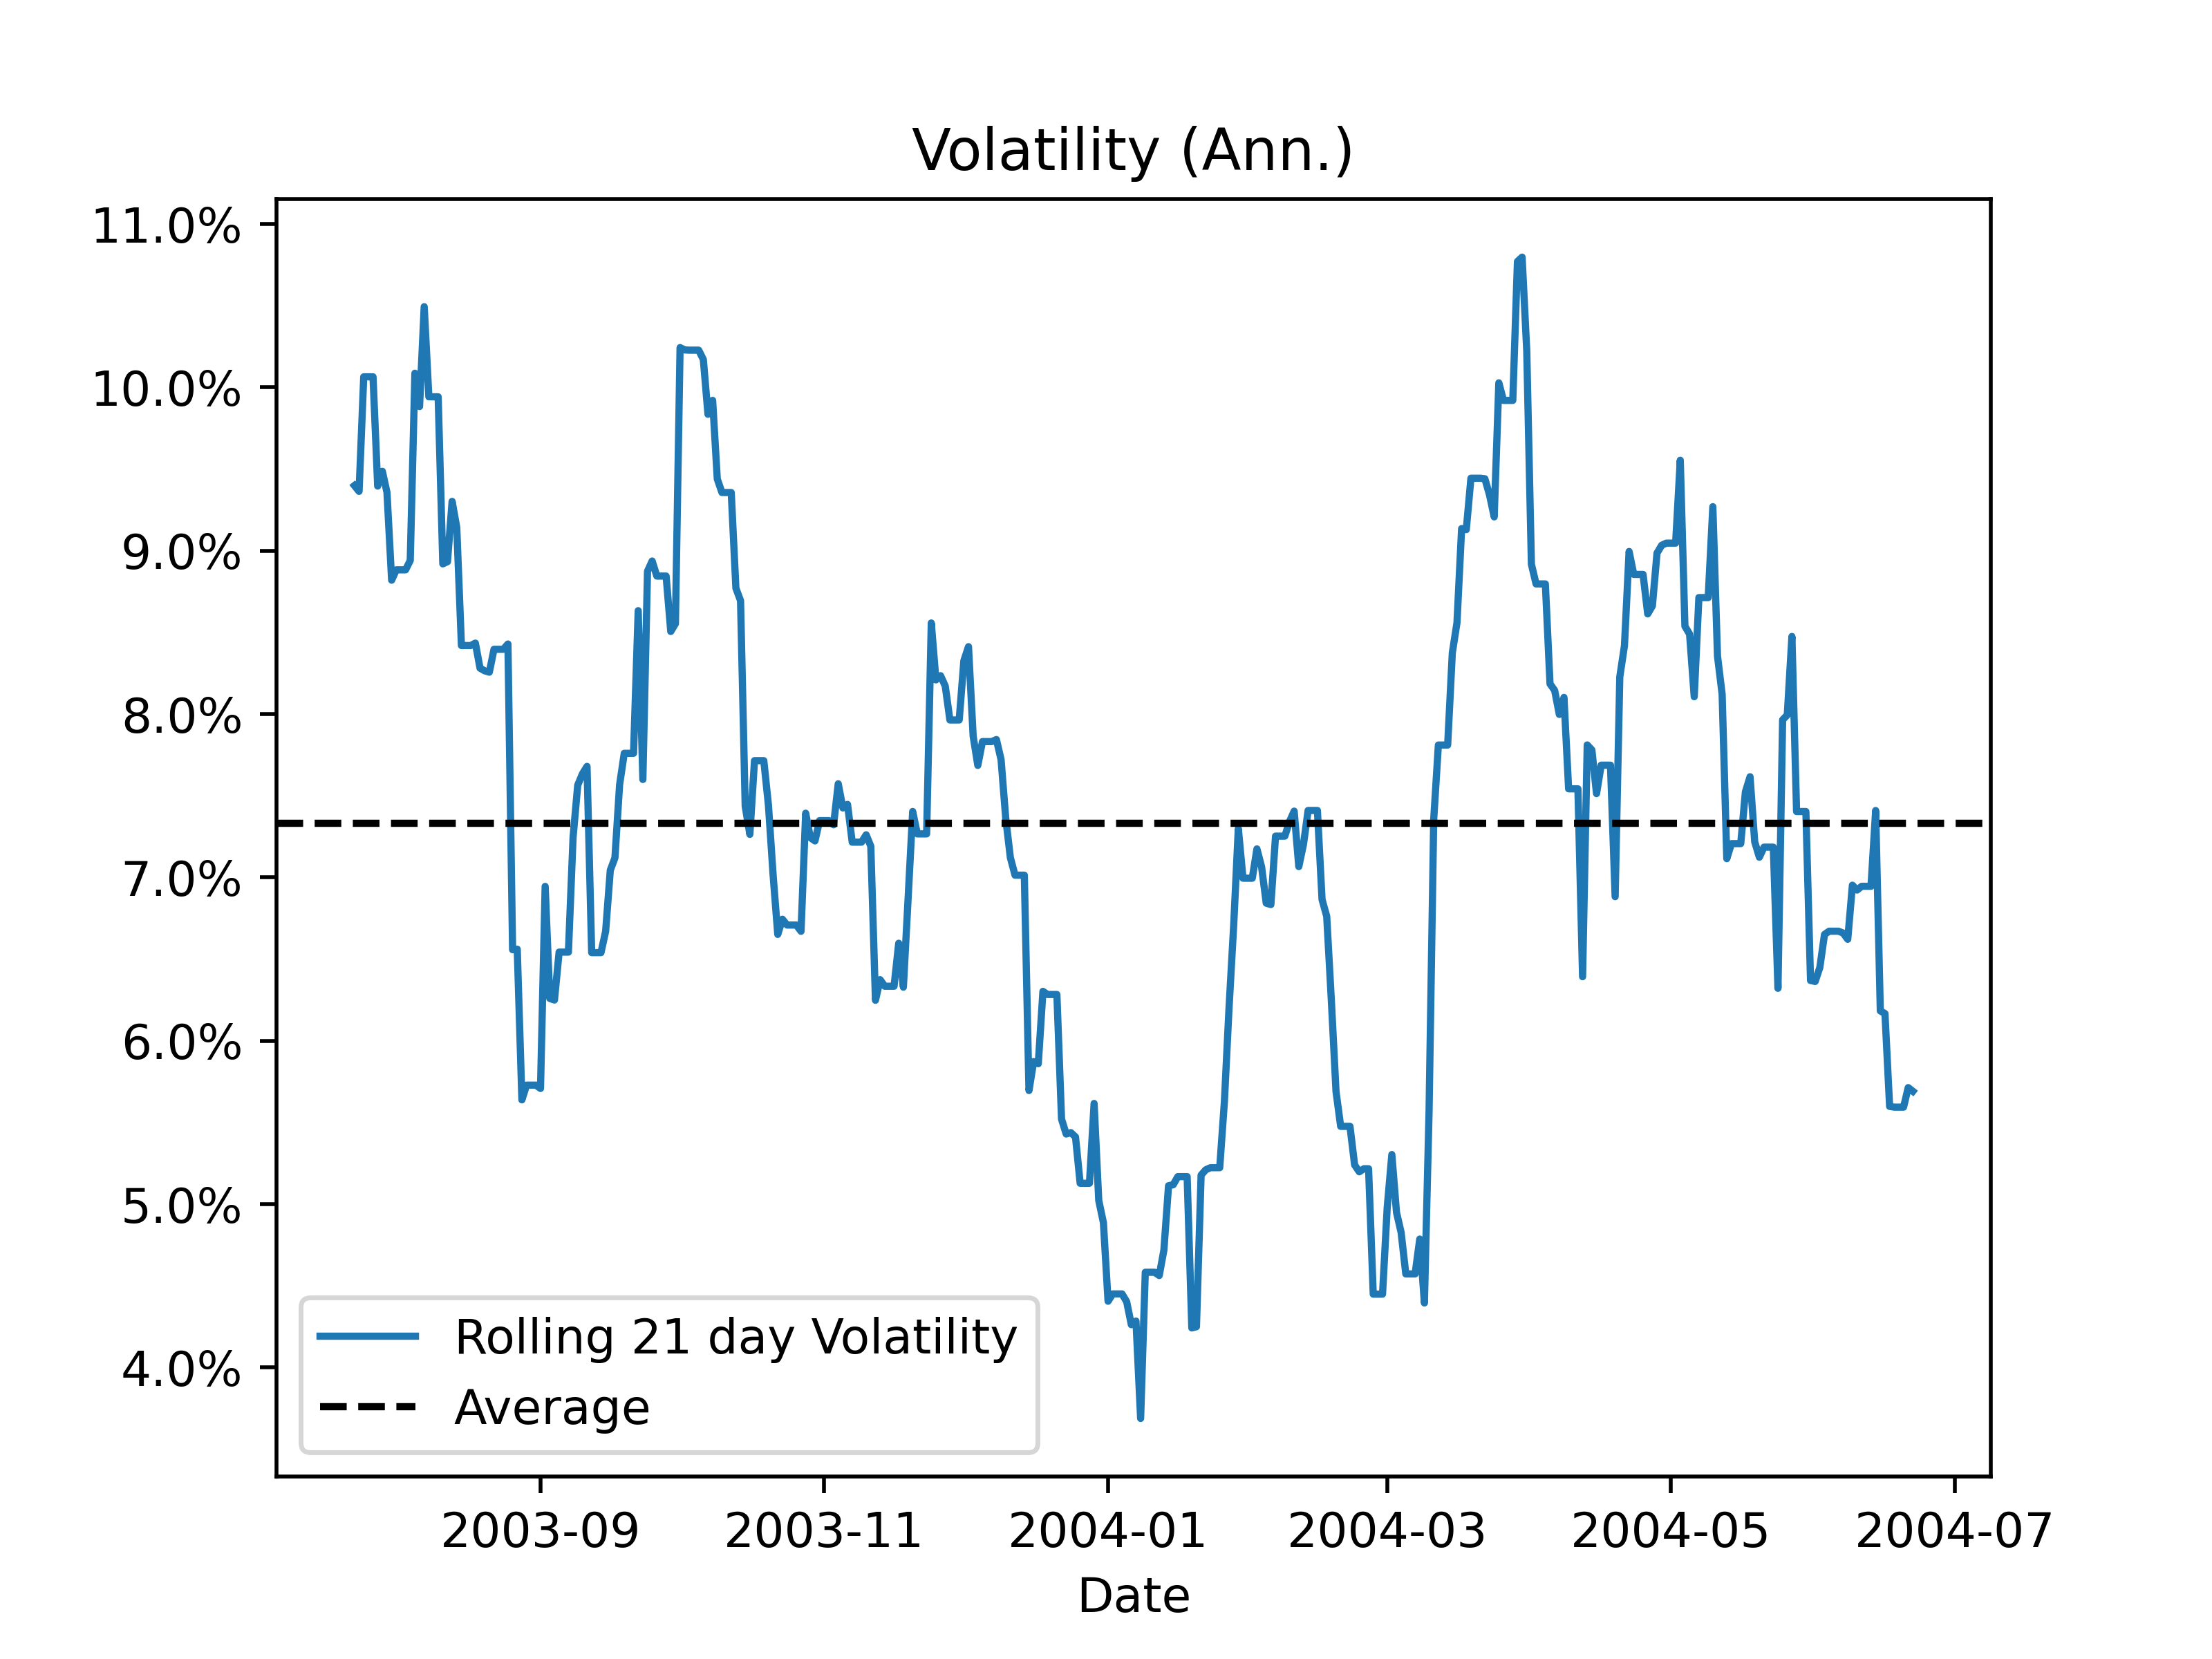
\includegraphics[width=0.7\linewidth]{./figures/volatility.png}
\caption{Volatility of the default portfolio with 0.3\% transaction costs; daily rebalancing.}
\label{figure:Task volatility}
\end{figure}

\subsection{Momentum Portfolio}

In addition to the default weights provided. I implemented a simple long-only momentum strategy using the same assets to demonstrate the flexibility of my backtester.

In brief, my momentum strategy puts the full allocation into the asset with the highest mean daily returns in the penultimate month before the current month (as is standard in the literature). For example, if we rebalance on August 1st, we long the stock with the best mean daily returns in June (not July). As this is not possible for the first two months in the dataset, I take the default weights provided for these months. In months where the returns are all negative, I hold cash. A long-short strategy could also be used to manage risk, although this doesn't perform as well here and both methods are dubious anyhow with only 5 assets to pick from.

Table~\ref{table:mom} and Figures~\ref{figure:Mom NAV}, \ref{figure:Mom underwater}, \ref{figure:Mom volatility} show the statistics from this simple momentum strategy. I avoid discussions to keep this report brief.


\begin{table}[p]
\centering
\caption{Momentum portfolio performance summary; daily rebalancing.}
\label{table:mom}
\begin{tabular}{rrrrrrr}
\toprule
\midrule
Transaction Cost & 0.30\% \\
Risk Free Rate & 0.00\% \\
\hline
Total Return & 38.47\% \\
Return (Ann.) & 25.83\% \\
Sharpe Ratio & 1.32 \\
Sharpe Ratio (Ann.) & 1.11 \\
Volatility (Ann.) & 23.22\% \\
Max Drawdown & 18.15\% \\
Max Drawdown Date & 2004-05-19 \\
Longest Drawdown (Days) & 107 \\
\bottomrule
\end{tabular}
\end{table}


\begin{figure}
\centering
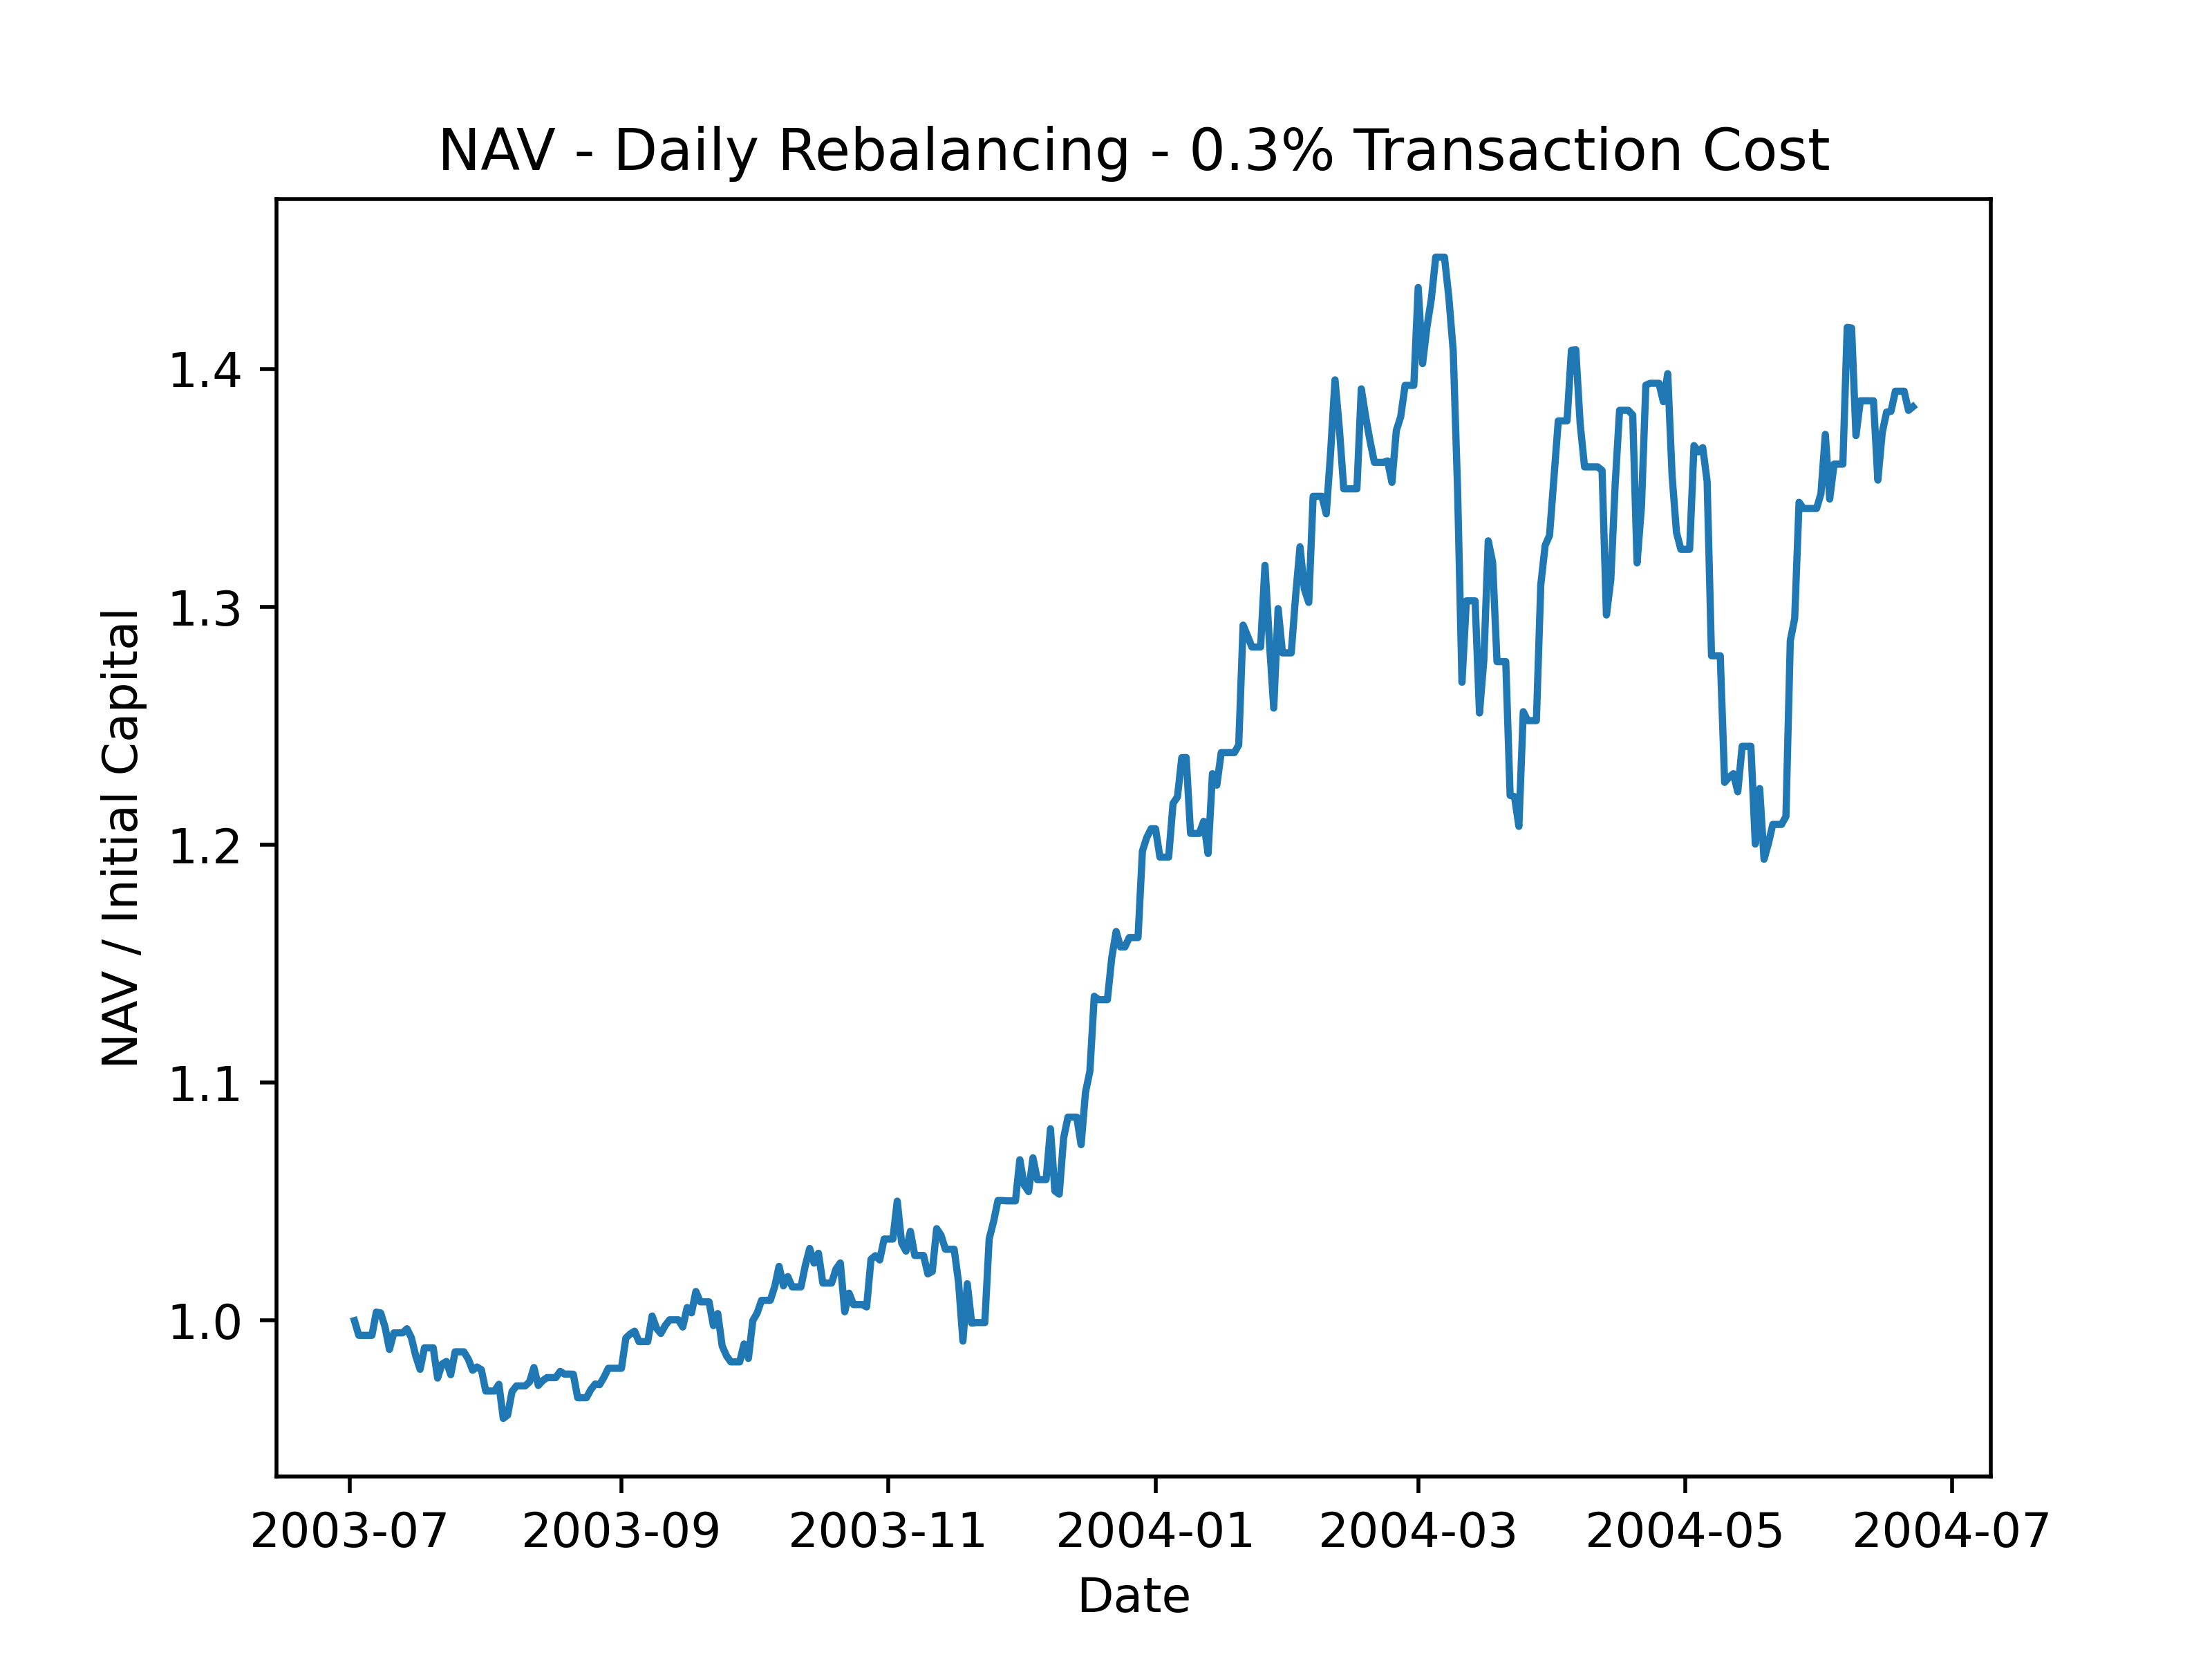
\includegraphics[width=0.7\linewidth]{./figures/nav_mom.png}
\caption{Net asset value of momentum portfolio with 0.3\% transaction costs; daily rebalancing.}
\label{figure:Mom NAV}
\end{figure}

\begin{figure}
\centering
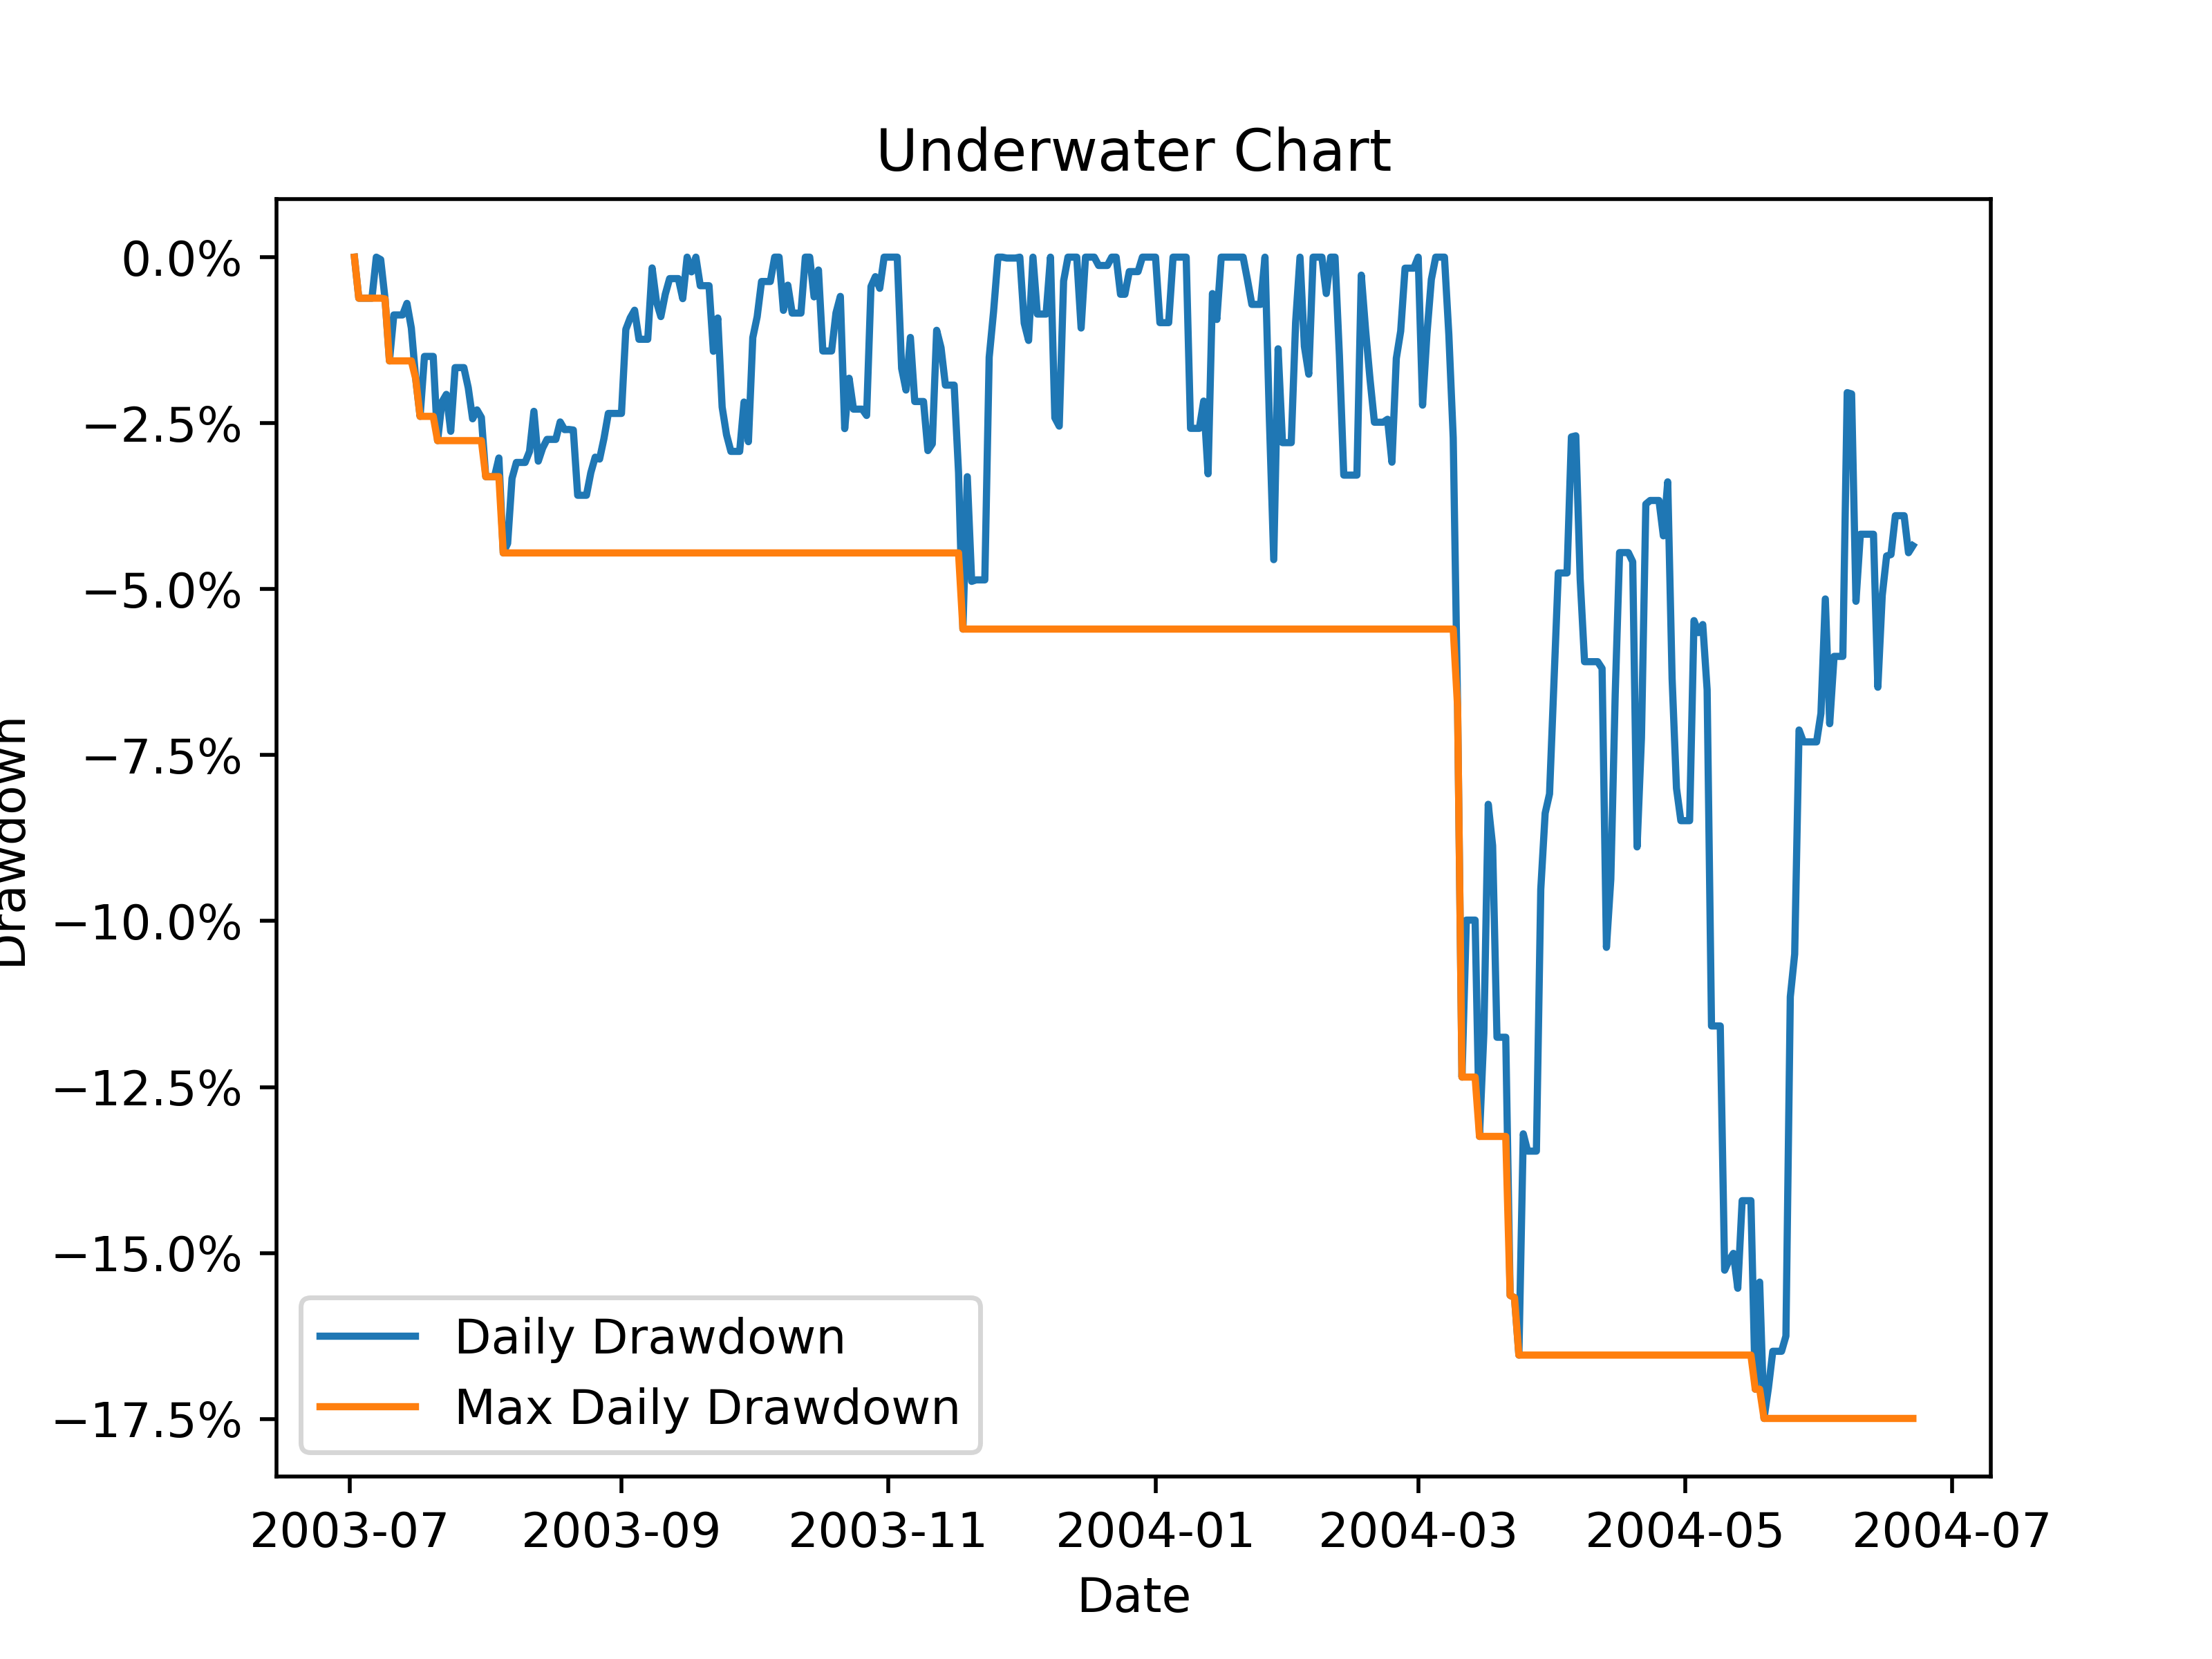
\includegraphics[width=0.7\linewidth]{./figures/underwater_mom.png}
\caption{Drawdowns of the momentum portfolio with 0.3\% transaction costs; daily rebalancing.}
\label{figure:Mom underwater}
\end{figure}

\begin{figure}
\centering
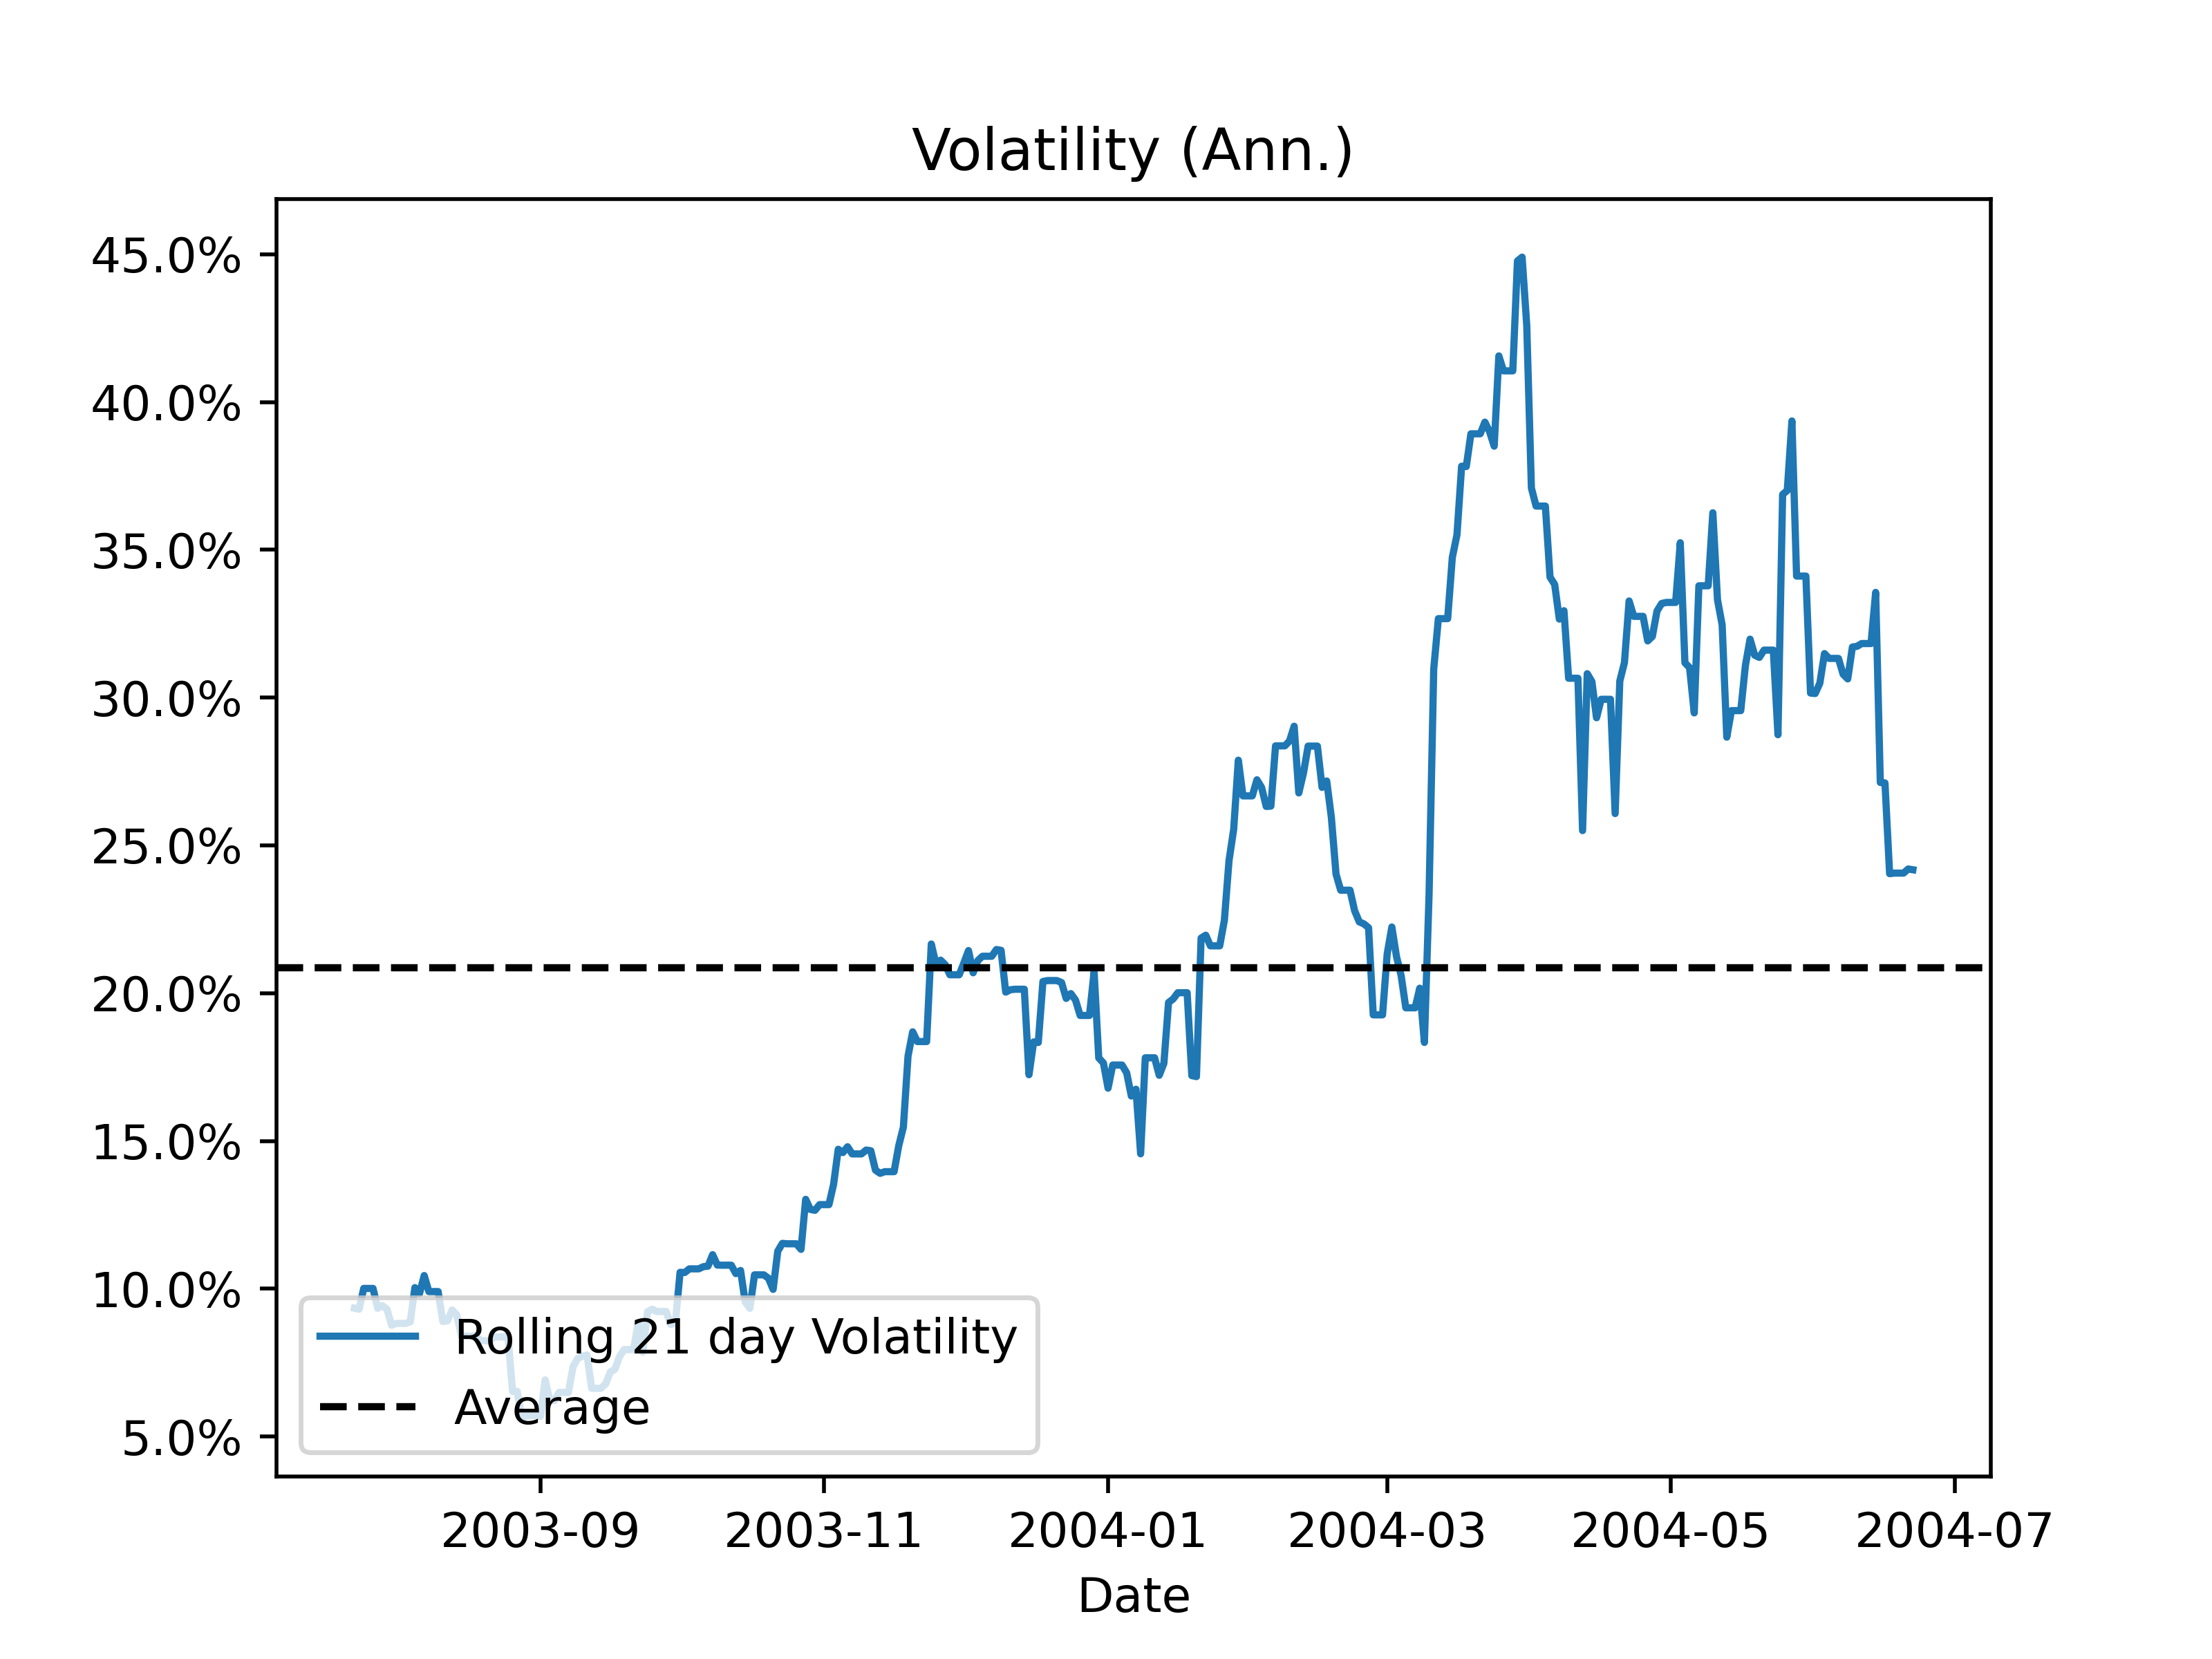
\includegraphics[width=0.7\linewidth]{./figures/volatility_mom.png}
\caption{Volatility of the momentum portfolio with 0.3\% transaction costs; daily rebalancing.}
\label{figure:Mom volatility}
\end{figure}





\end{document}
